%----------------------------------------------------------------------------------------------------------------------------------------------------------%
\chapter{Computational experimentation}
%----------------------------------------------------------------------------------------------------------------------------------------------------------%
\epigraph{Remember that all models are wrong; the practical question is how wrong do they have to be to not be useful.}{\textit{Norman Richard Draper}}
%----------------------------------------------------------------------------------------------------------------------------------------------------------%
\section{Description}
\paragraph{}This second experiment looks at computing the shape of a \emph{Staphylococcus aureus} P-68 bacteriophage starting from its DNA sequence. This will analyze the process of protein translation, as well as looking at the process of using AlphaFold\cite{jumperHighlyAccurateProtein2021}. To compute the secondary, tertiary and quaternary structures of the proteic parts of the virus we will use the Google CoLaboratory version of AlphaFold\cite{GoogleColaboratoryAlpha1970}, as it allows for far more computer power than available on a simple laptop.
%----------------------------------------------------------------------------------------------------------------------------------------------------------%
\section{Protocol followed}
The protocol followed is very simple, as AlphaFold, the Artificial Intelligence model used does the hardest part of the work for us:
\begin{enumerate}[label=\arabic*)]
\item Convert the DNA sequence of one of the proteins to an mRNA sequence, by taking into account the fact that there's base complimentariety.
\item Convert the mRNA sequence to an aminoacid sequence of the proteins by using the genetic universal code table.
\item Feed the aminoacid sequences to AlphaFold, obtain the models for each protein.
\item Assemble the bacteriophage. 
\item Print, polish and paint a 3D physical model of the bacteriophage to illustrate better how it functions.
\end{enumerate}
The AlphaFold Jupiter notebook\cite{GoogleColaboratoryAlpha-} used is optimized for use with the NVIDIA Tesla T4 computing engine GPU, an extremely powerful graphics card, like the ones used in computers to render extremely detailed polygons in videogames or 3D animations. That's the one I used when folding\footnote{Folding a protein: calculating, by using the theorical intermolecular forces, the shape of the protein} the proteins. The genomic sequence used is NC\_004679.1, which leads to the PDB structure 6Q3G.
%----------------------------------------------------------------------------------------------------------------------------------------------------------%
\section{Results and analysis}
The gene codified for a total of 22 separate proteins. After BLASTing\footnote{BLAST: digital service that takes a sequence of DNA in the FASTA format and attempts to find the organism and/or protein that it codifies} all of them, I got the following list:
\begin{center}\begin{figure}[H]\centering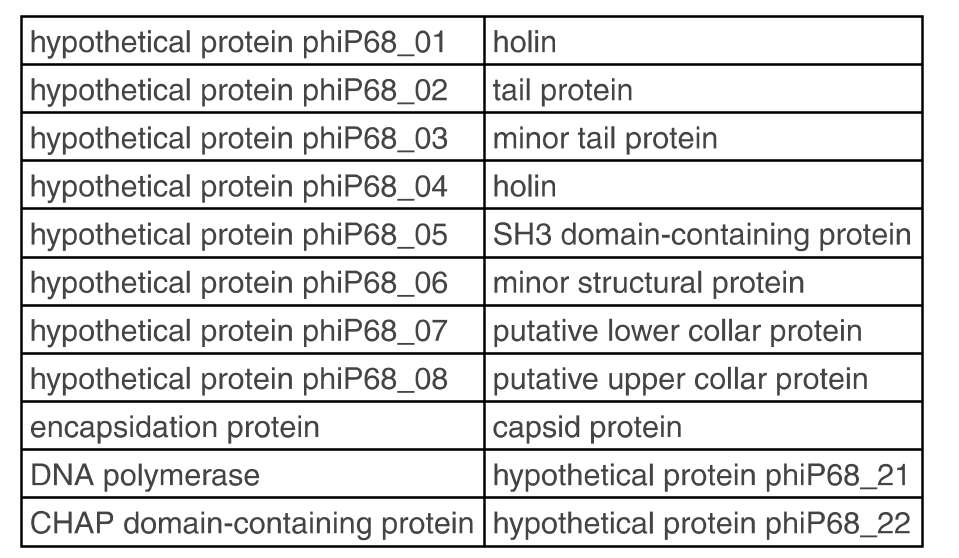
\includegraphics[width=0.90\textwidth]{AF3.png}\end{figure}\end{center}
Which then assembled into the following figure:
\begin{center}\begin{figure}[H]\centering\includegraphics[width=0.90\textwidth]{p68.png}\end{figure}\end{center}
These three views allow us to see the capsid, the collar and sheath, the tail fibers, and the spikes, which are integrated into the collar. The tail fibers act exactly like the Coronavirus spike proteins: they bind to a specific compound on the surface of the bacteria, but they don't access it. They only bind to the surface, perforate it using the spikes and then, due to a difference in pressures, the genetic material is expulsed into the cell. Then, it uses the fact that bacteria will integrate strands of genetic material floating in the environment into its own hereditary material in order to force the host to reproduce the virus.
\paragraph{}Using the PDB2STL pymol\footnote{Pymol: program that takes a protein database and converts it into a viewable model} tool, I managed to create a printable 3D model of the virus, which was then polished using a wire brush and painted gray so the details can be seen with more clarity. Then, a white filament strand was added to symbolize the genetic material being oozed into a cell:
\begin{center}\begin{figure}[H]\centering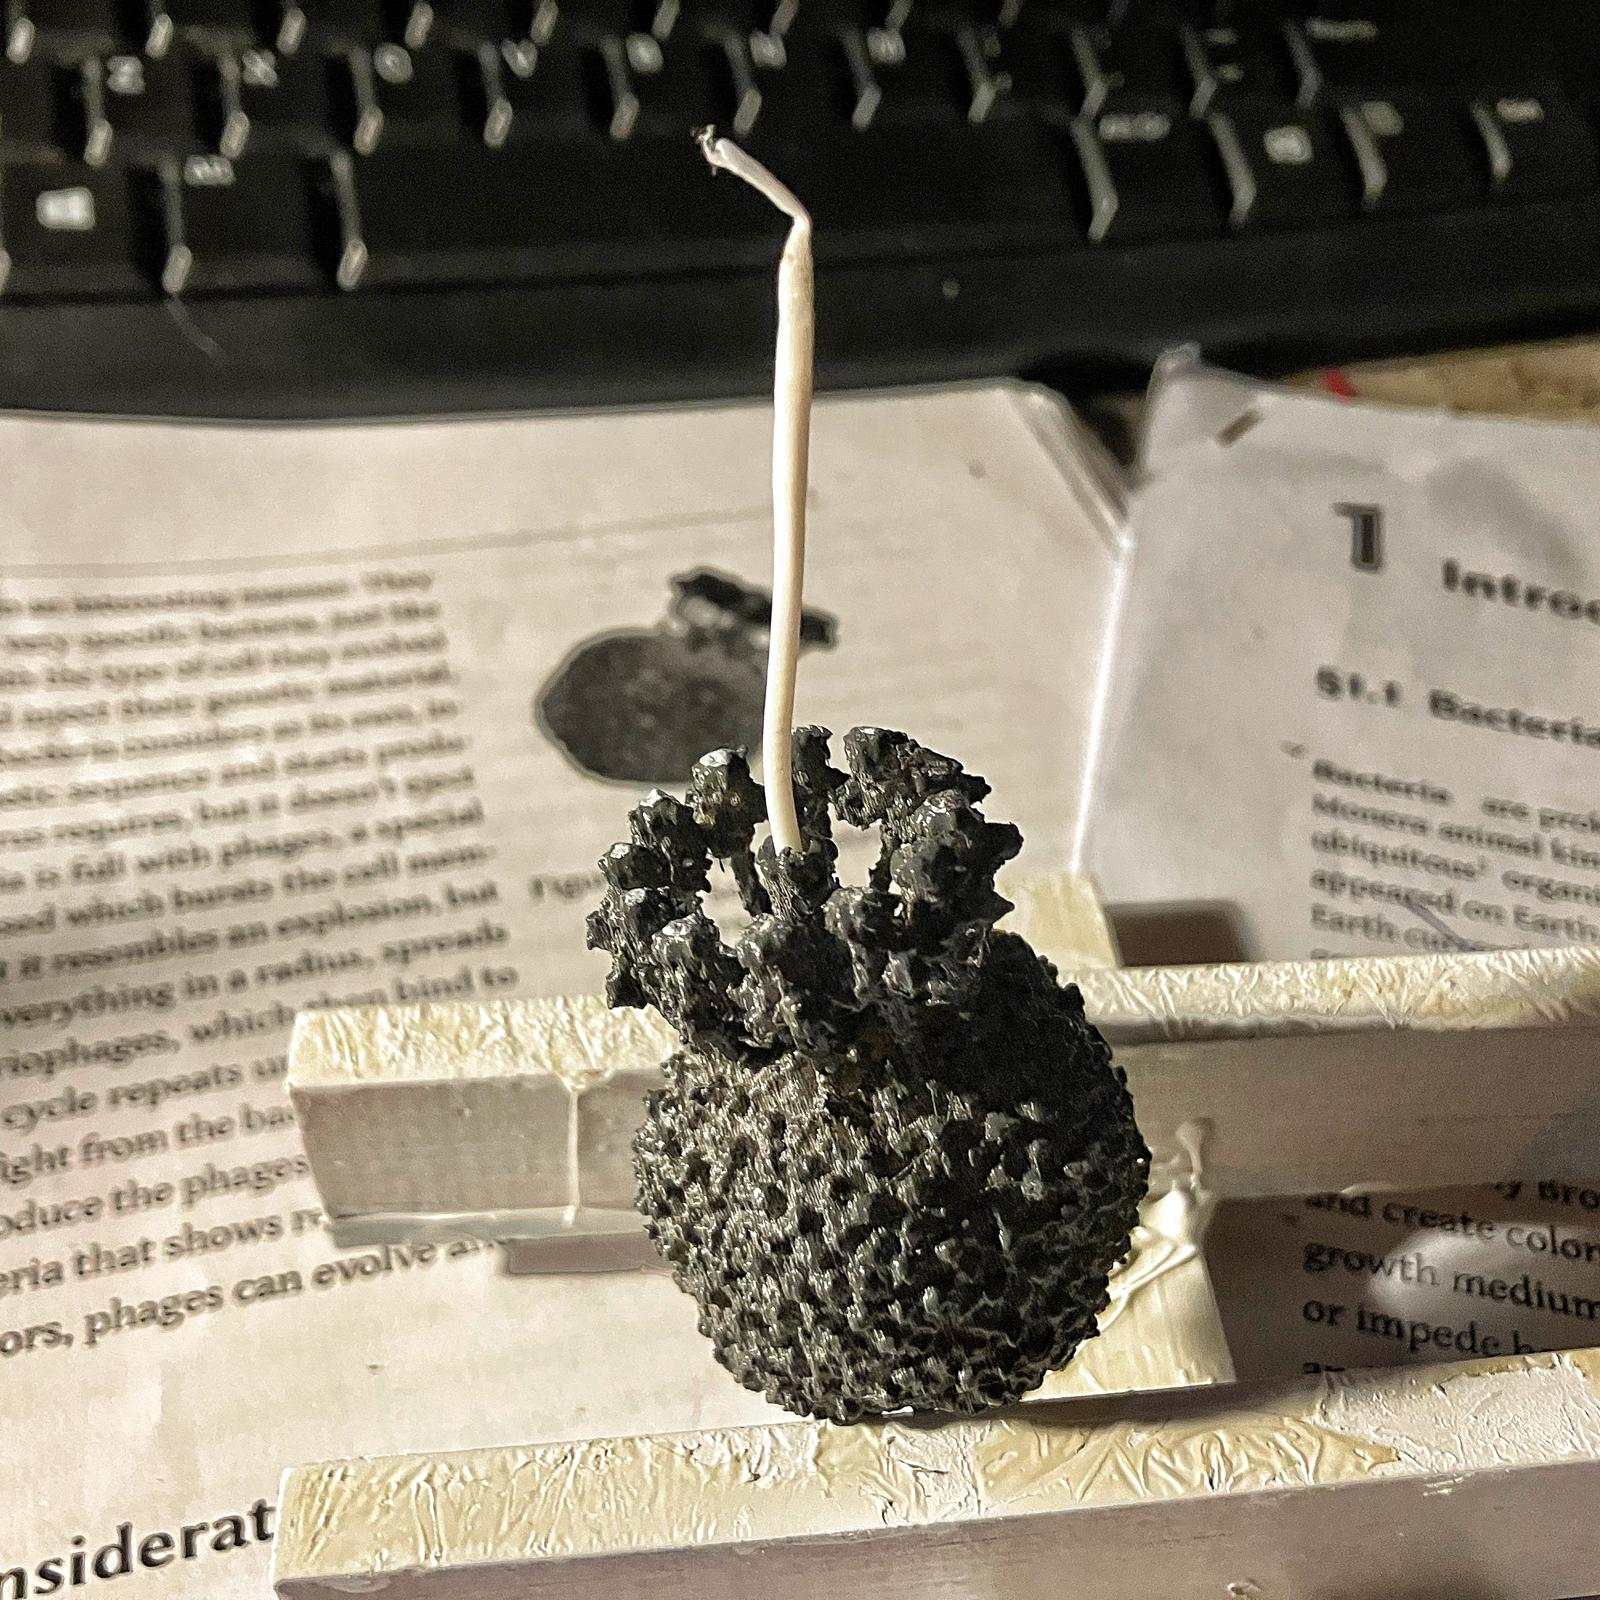
\includegraphics[width=0.50\textwidth]{3dirl.jpg}\end{figure}\end{center}